\documentclass{article}

\usepackage{Sweave}
\begin{document}
\Sconcordance{concordance:probabilities4.tex:probabilities4.Rnw:%
1 2 1 1 0 22 1 1 17 3 0 1 2 2 0 1 2 2 0 1 3 2 0 2 3 3 1 1 8 1 3 6 1 1 %
16 3 0 1 2 2 0 1 2 2 0 1 2 2 0 1 2 2 0 1 4 1 3 3 1 1 8 1 3 4 1}


\title{Probabilities of significance for false null-hypotheses}

\author{Mc}
\maketitle
\section*{Introduction}
In simulations we checked the propability of an indicator (continuous or media-split) as the probability (frequency of runs) of being nonsignificant when it should not be (latent effect size is greater than zero) and then the probability of being significant when it should be .
\section*{Setup}
\subsection*{Model}
Two continuous latent variables (\(\eta\) and \(\xi\) ) are created with N cases, sharing a correlation equal to \(\rho\). A measure \(x\) of \(\xi\) is created with reliability \(rel\), and then  is dichotomized accordingly to \(p\) \(1-p\) into \(c\). The correlations \( r_pe=r(\eta,x) \)  and \( r_pb=r(\eta,c) \) are computed, their p-value and significance (at .05) is recorded.
\subsection*{Design}
\(\rho=(0,.1,.2,.3,.4,.5,.6,.7) \)
\(rel=(0.3, 0.4 ,0.5, 0.6, 0.7 ,0.8 0.9) \) 


\subsection*{Propabilities of nonsignificant tests for  \(\rho\)>0}

Here we compute the proportions of runs in which we have a nonsignificant result on either or both of the tests and \(\rho\)>0
The probabilities are the following: \(f_1\) is the number of times the indicator was the only one nonsignificant (so the other was ) for a given \(\rho\), \(f_t\) is the number of runs for a given \(\rho\). The probability \(P\) is \(P=f_1 / f_t \))  


\begin{Schunk}
\begin{Soutput}
Probability of only Categorical as nonsignificant
\end{Soutput}
\begin{Soutput}
[1] 0.05500000 0.11257143 0.14928571 0.16157143 0.13300000 0.11514286 0.09771429
\end{Soutput}
\begin{Soutput}
Probability of  only Continuous was nonsignificant
\end{Soutput}
\begin{Soutput}
Probability of  both  nonsignificant
\end{Soutput}
\end{Schunk}


\subsubsection*{Figure 1: Probabilities of nonsignificant tests under false null-hypothesis}

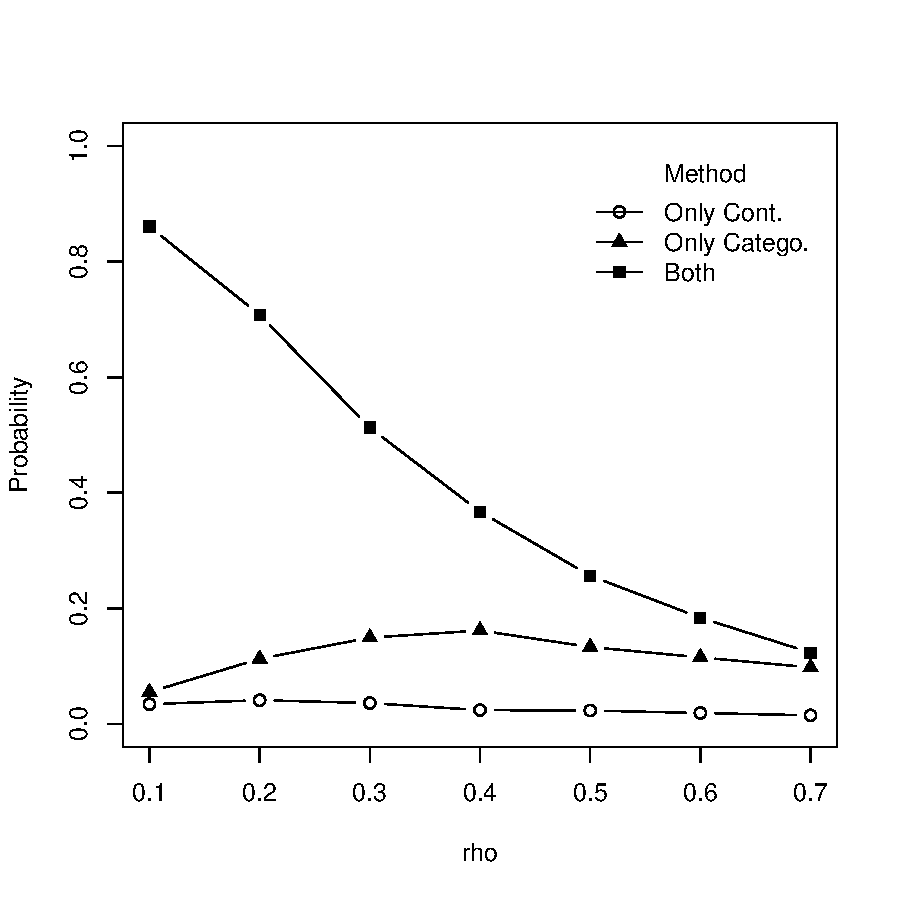
\includegraphics{probabilities4-dd}



\subsection*{Propabilities of being significant as a functions of \(\rho\)}

The probabilities are the following: \(f_1\) is the number of times the indicator was the only one significant (so the other was not) for a given \(\rho\), \(f_t\) is the number of runs for a given \(\rho\). The probability \(P\) is \(P=f_1 / f_t \))  

\begin{Schunk}
\begin{Soutput}
Probabilites only Continuous was significant under the null hypothesis
\end{Soutput}
\begin{Soutput}
[1] 0.05500000 0.11257143 0.14928571 0.16157143 0.13300000 0.11514286 0.09771429
\end{Soutput}
\begin{Soutput}
Probabilites of only Categorical significant under true hypotheses
\end{Soutput}
\begin{Soutput}
[1] 0.03414286 0.04100000 0.03600000 0.02385714 0.02314286 0.01885714 0.01485714
\end{Soutput}
\begin{Soutput}
Probability of  both  significant
\end{Soutput}
\end{Schunk}


\subsubsection*{Figure 2: Probability of being significant}

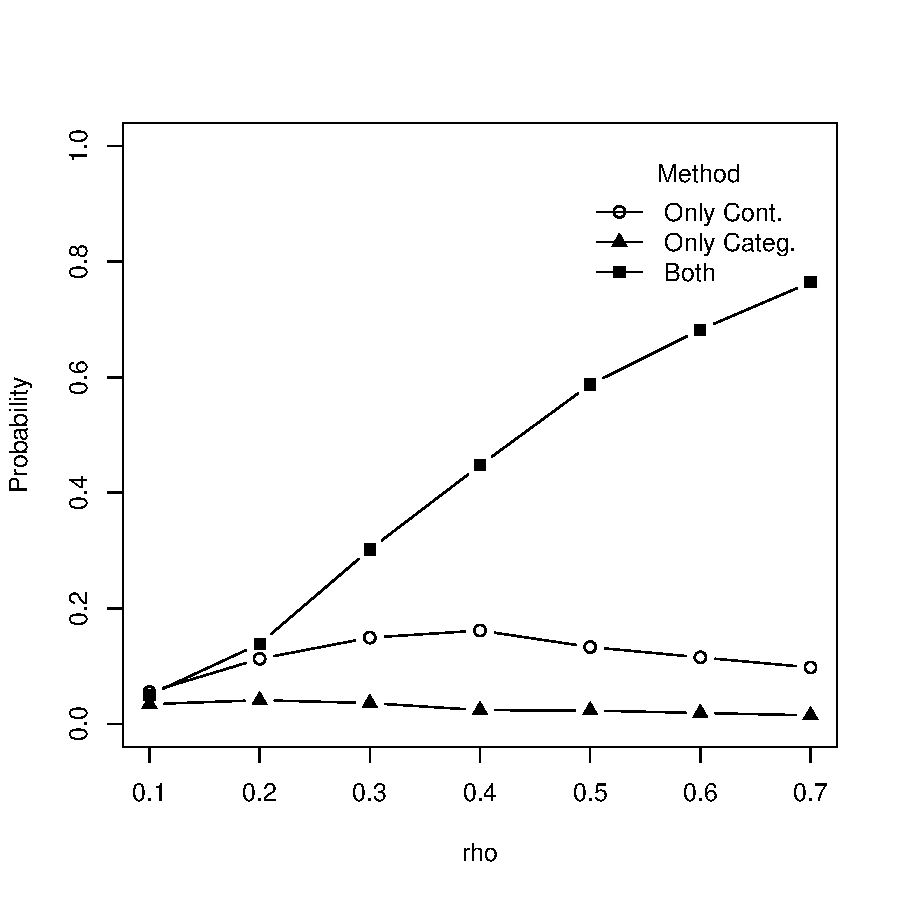
\includegraphics{probabilities4-bb}




\end{document}
